\documentclass{astroedu-lab}

\begin{document}

\pagestyle{plain}

\begin{problem}{\huge Лабораторная работа 2.2.1\\\\Исследование взаимной диффузии\\\\газов\\\\Выполнил Жданов Елисей Б01-205}

\section{Цель работы:}

1) Регистрация зависимости концентрации гелия в воздухе от времени с помощью датчиков теплопроводности при разных начальных давлениях смеси газов

2) Определение коэффициента диффузии по результатам измерений

\section{Оборудование:}

Измерительная установка

Форвакуумный насос

Баллон с гелием

Манометр

Источник питания

Магазин сопротивлений

Гальванометр

Секундомер

\section{Теоретическая справка}

Скорость диффузии определяется коэффициентом диффузии, а именно пропорциональна ему. С длиной свободного пробега и средней скоростью он связан как

\begin{equation}
	D = \frac{1}{3} \lambda \overline{v}
\end{equation}

Также запишем выражение для средней скорости

\begin{equation}
	\overline{v} = \sqrt{\frac{8 R T}{\pi \mu}}
\end{equation}

и длины свободного пробега

\begin{equation}
	\lambda = \frac{1}{n \sigma}
\end{equation}

Интегрируя дифференциальное уравнение диффузии, получим соотношение

\begin{equation}
	\Delta n = \Delta n_0 e^{-t/\tau}
\end{equation}

где

\begin{equation}
	\tau = \frac{V L}{2 S D}
\end{equation}

Построив соответствующий логарифмическим координатам линеаризованный график, получим из него коэффициент диффузии.

\section{Экспериментальная установка}

\begin{figure}[!h]
	\centering
	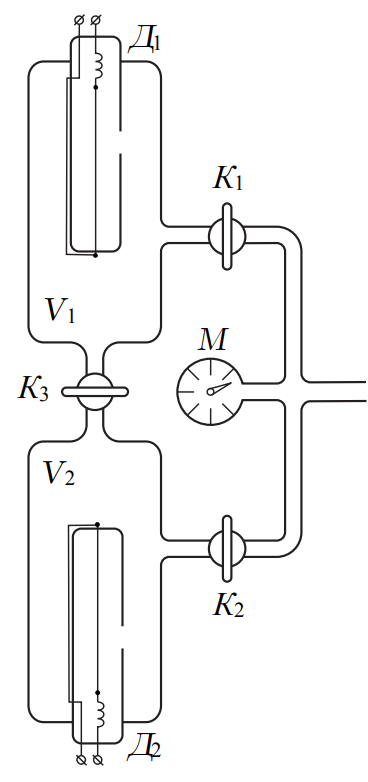
\includegraphics[width=0.2\textwidth]{установка.png}
	\label{fig:boiler}
\end{figure}

Выравнивание давлений в сосудах V1 и V2 без изменения состава газов в них может быть осуществлено через обводные трубки посредством кратковременного открытия кранов К1 и К2 (при закрытом К3).

Балансировку показаний вольтметра необходимо производить перед каждым измерением, потенциометром.

\section{Измерения, Обработка}

1-2) Убедимся, что установка настроена и будем выполнять все действия согласно инструкции. На используемой установки нет возможности сброса давления в насосе после откачки, остальное соответствует методике эксперимента.

\begin{center}
	\Large Зависимость напряжения от времени V(t)
\end{center}

\begin{figure}[!h]
	\centering
	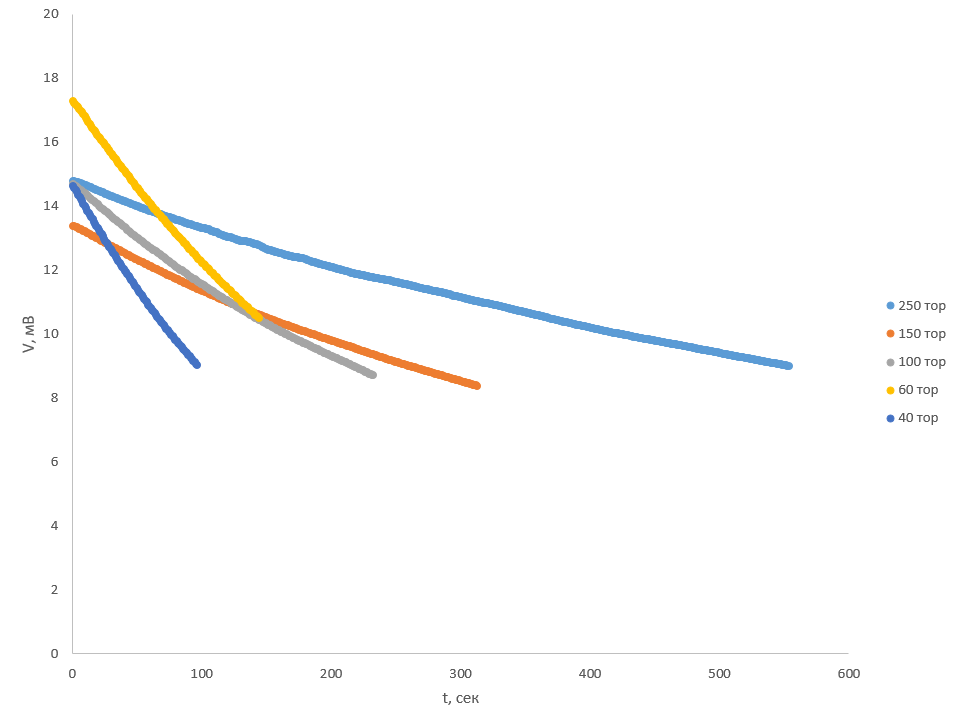
\includegraphics[width=1\textwidth]{линейный.png}
	\label{fig:boiler}
\end{figure}

2-6) //Специфика//

В результате проведения эксперимента были получены данные в формате .csv, которые прилагаются к работе.

Запишу в таблицу уточненные по результатам смешивания получанные давления

За вакуум приму давление 101.25 кгс/см$^2$ на манометре.

\begin{center}
\begin{tabular}{|c|c|}
\hline 
$p_\text{прибор}$, кгс/см$^2$ & P, тор \\
\hline
96.0 & 38.7 \\
93.4 & 57.8 \\
87.8 & 99.1 \\
80.6 & 152 \\
67.2 & 251 \\
\hline
\end{tabular}
\end{center}

Погрешность полученного давления в торах определяется погрешностью замера давления на манометре 0.2 кгс/см$^2$ и составляет 1.5 тор для каждого опыта.

Построю графики зависимости $ln(V)$ от $t$.

\begin{center}
	\Large Зависимость $ln(\frac{V}{V_0})[t]$
\end{center}

\begin{figure}[!h]
	\centering
	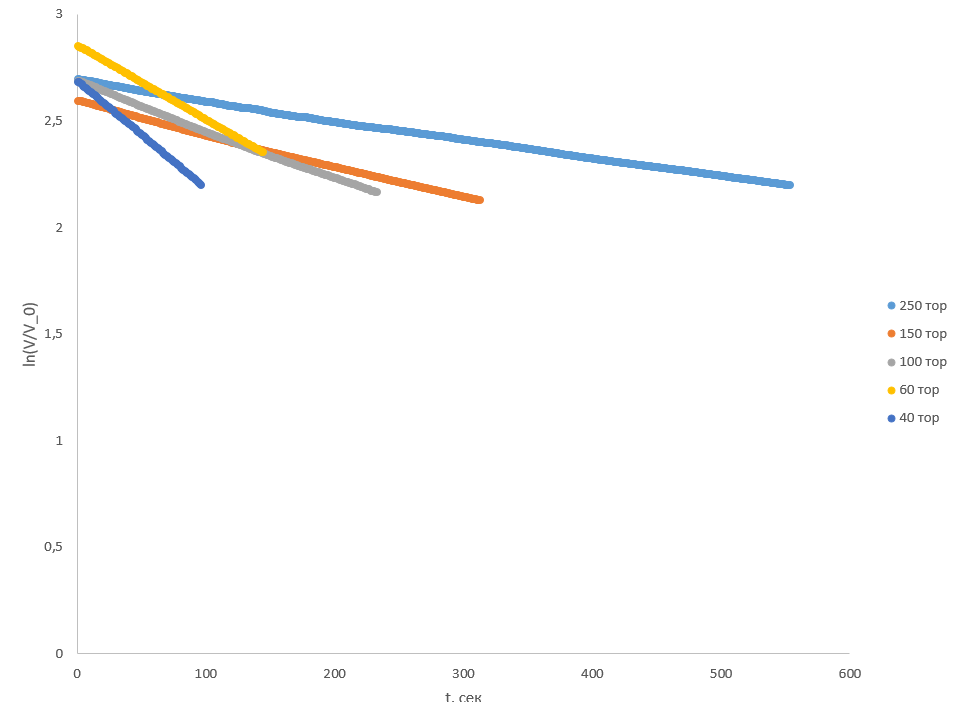
\includegraphics[width=1\textwidth]{логарифм.png}
	\label{fig:boiler}
\end{figure}

Найдем угловые коэффициенты прямых для каждого опыта по МНК.

\[
	a = \frac{<x_i y_i> - < x > < y_i >}{< x_i^2> - < x_i >^2}
\]

\[
	b = < \nu_i > - a < N_i >
\]

Также рассчитаем их погрешности

\begin{equation}
	S_a^2 = \frac{< x_i^2>}{< x_i^2 > - < x_i >^2} \cdot \frac{<  b_i - b > ^2}{n - 2}
\end{equation}


Запишем в таблицу коэффициенты наклона, полученные из МНК

\begin{center}
\begin{tabular}{|c|c|}
\hline 
P, тор & k, сек$^{-1}$ \\
\hline
250 & $(-0.0008823 \pm 0.0000015)$ \\
150 & $(-0.0014951 \pm 0.0000035)$ \\
100 & $(-0.0022635 \pm 0.0000058)$ \\
60 & $(-0.0034908 \pm 0.000001)$ \\
40 & $(-0.0050658 \pm 0.0000023)$ \\
\hline
\end{tabular}
\end{center}

Пересчитаю по формуле для коэффициента диффузии полученные значения k, обратные характерному времени $\tau$ в показателе экспоненты. Будем считать по указанию $L/S = (5.3 \pm 0.1)$ см$^{-1}$, а средний объем одного сосуда $V = 775 \pm 10$ см$^{3}$.

\begin{equation}
	D = -\frac{1}{\tau} \cdot \frac{L}{S} \cdot \frac{-V}{2} = -k \frac{L}{S} \frac{V}{2}
\end{equation}

Относительная погрешность D равна сумме относительных погрешностей коэффициента наклона, отношения L/S и объема соответственно.

Запишу значения в таблицу

\begin{center}
\begin{tabular}{|c|c|}
\hline 
P, тор & D, м$^{2}$/сек \\
\hline
250 & $(1.81 \pm 0.06) \cdot 10^{-4}$ \\
150 & $(3.07 \pm 0.11) \cdot 10^{-4}$ \\
100 & $(4.65 \pm 0.16) \cdot 10^{-4}$ \\
60 & $(7.2 \pm 0.2) \cdot 10^{-4}$ \\
40 & $(10.4 \pm 0.3) \cdot 10^{-4}$ \\
\hline
\end{tabular}
\end{center}

Построим график зависимости коэффициента диффузии от 1/P

\newpage

\begin{center}
	\Large Зависимость D от 1/P
\end{center}

\begin{figure}[!h]
	\centering
	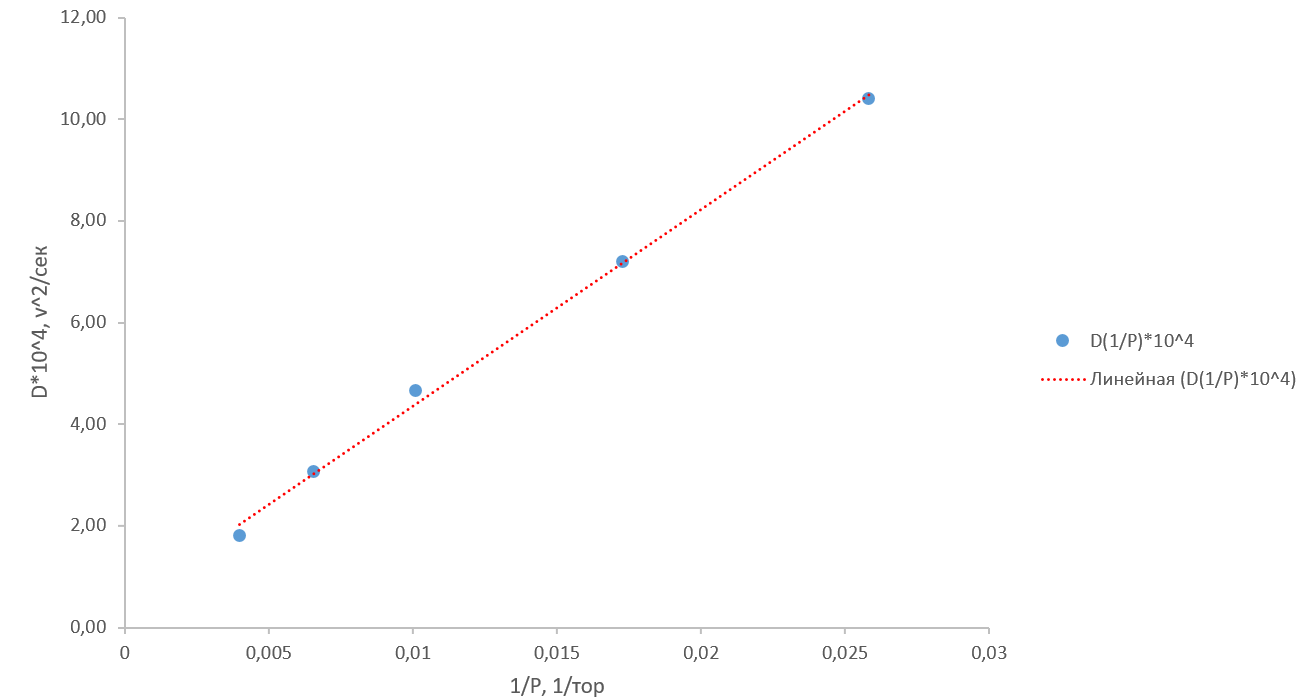
\includegraphics[width=1\textwidth]{лол.png}
	\label{fig:boiler}
\end{figure}

С помощью МНК определим зависимость

\begin{equation}
	D = (0.49 \pm 0.17) + \frac{(387 \pm 11)}{P}
\end{equation}

Для атмосферного давления D составит $(1.00 \pm 0.18)$ м$^2$/сек

Табличное же значение 0.66 м$^2$/сек.

Из полученного значения D, рассчитав среднюю скорость молекул при комнатной температуре $\overline{v} = \sqrt{\frac{8 R T}{\pi \mu}} = 1257$ м/c, получим 

\begin{equation}
	\lambda = \frac{3 D}{\overline{v}} = 240 \pm 40 нм
\end{equation}

И наконец

\begin{equation}
	\sigma = \frac{k T}{p \lambda} = (4.59 \pm 0.08) \cdot 10^{-20} \text{м}^2
\end{equation}

%\begin{figure}[!h]
%	\centering
%	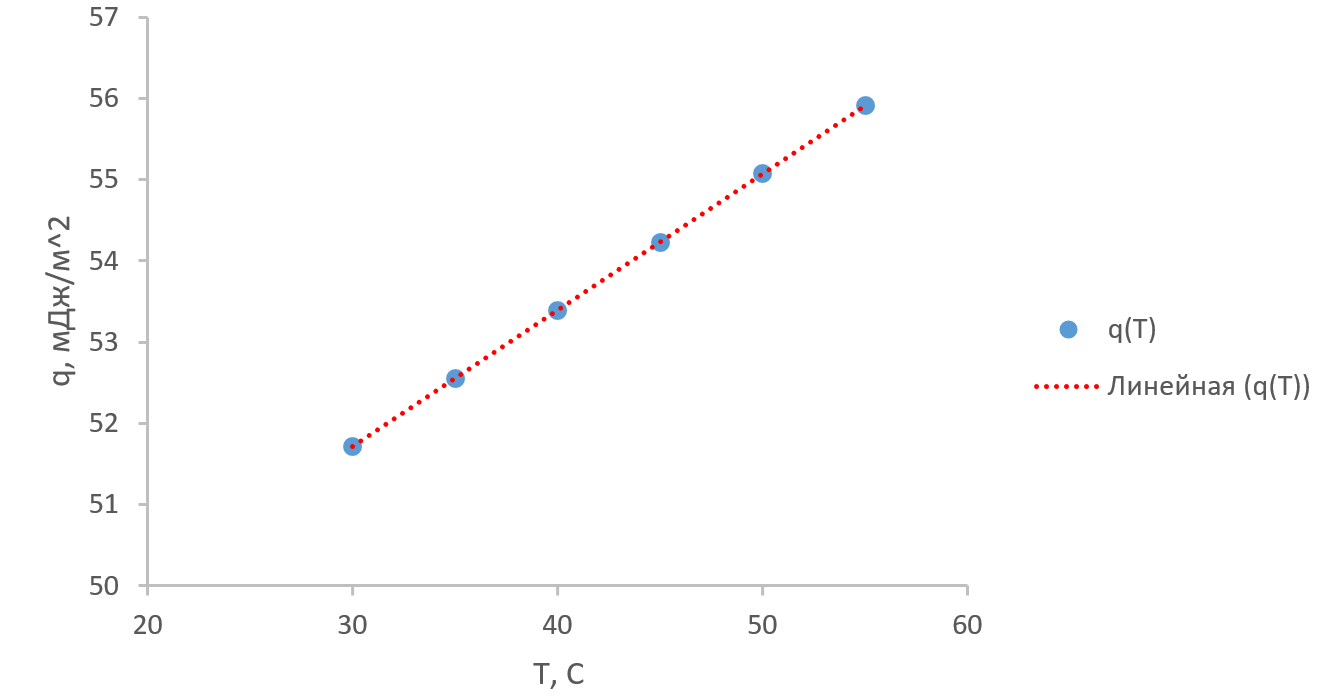
\includegraphics[width=1\textwidth]{2023-02-23_22-23-59.png}
%	\label{fig:boiler}
%\end{figure}

\section{Вывод}
Данные сходятся с табличными в пределах погрешности, лаба замечательная.

\section{Ресурсы}

Расчет по МНК: метод-наименьших-квадратов.рф


\end{problem}
\end{document}
